%!TEX  TS-program = xelatex
\documentclass[12pt]{article}

\usepackage{xeCJK}
\linespread{1.5} % 1.5倍行距
\usepackage{graphicx}
\usepackage{subfigure}

\title{Learn to use \LaTeX}
\author{hank}
\date{\today}

\begin{document}

\maketitle

\section{Ubuntu下\LaTeX 安装及中文配置}
\subsection{首先安装texlive-latex-base}

使用命令\ 
\fbox{
	sudo apt-get install texlive-latex-base
}

\subsection{然后安装中文支持包latex-cjk-all}

使用命令\ 
\fbox{
	sudo apt-get install latex-cjk-all
}

\subsection{安装texlive-xetex以使用xelatex编译中文}

使用命令\ 
\fbox{
	sudo apt-get install latex-xetex
}

\subsection{编译\ .tex文件}

打开编辑器,编辑并保存一个\ .tex文件。这里要注意,保存好的\ .tex文件可以直接使用xelatex
\quad example.tex\ (example为你自己保存的文件名)来编译,如果出现报错缺失\
*.sty(*为缺失的\ .sty文件名称),可以使用\ 
\fbox{
	sudo apt-cache search *
}\ 来查找缺失的\ .sty文件所在的包。选择查找结果中的一个包,使用
\fbox{
	sudo apt-get install
}\ 命令来安装。

\subsection{vim下使用插件}

在vim下使用插件可以方便的实现预览, 我使用了Vundle
插件管理工具来安装。在\ \textasciitilde/.vimrc中加入以下内容:
	
\noindent Plugin `lervag/vimtex'\\
let g:vimtex\_latexmk\_options=`-pdf
-pdflatex=``xelatex-synctex=1$\backslash$\quad\%S$\backslash$\quad\%O"\quad-verbose\
-file-line-error\ -interaction=nonstopmode' \\
let g:tex\_flavor=`latex' \\
let g:vimtex\_view\_method=`zathura' \\
let g:vimtex\_quickfix\_mode=0 \\
set conceallevel=1 \\
let g:tex\_conceal=`abdmg' \\
let g:Tex\_CompileRule\_pdf = `xelatex -interaction=nonstopmode \$*' \\
然后在vim中输入命令\ \fbox{
	:PluginInstall
}\ 即可。未安装zathura可使用\ \fbox{
	sudo apt-get install zathura
}\ 安装zathura。在vim中编辑\ .tex文件完成后,
按ESC,在命令模式下直接输入\ $\backslash$ll即可实现预览pdf。若提示编译错误,
可使用\ $\backslash$le查看错误日志。

\textbf{注意:}若在vim下编译不通过,可尝试在\ .tex文件间头部
添加如下一行,将编译引擎设置为\ xelatex,然后重启vim即可。
\begin{center}
	\fbox{
		\%!TEX TS-program = xelatex	
	}
\end{center}

\subsection{自动补全YCM插件安装}
安装YouCompleteMe可以实现自动补全功能,不仅支持\LaTeX 语法,还支持其他编程语言,如C、
python等。使用Vundle插件管理,只需要在\textasciitilde/.vimrc中加入以下内容:
\begin{center}
	\fbox{
		Bundle\quad `Valloric/YouCompleteMe'
	}
\end{center}
\textbf{注意:}安装YCM前首先要确保依赖包安装了,使用下面的命令安装依赖包。\\
sudo apt-get install ctags \\
sudo apt-get install build-essential cmake python-dev \\
安装完成后启动vim,使用\ :BundleInstall来安装,完成后若提示\textbf{can
not find YCM core},只需要进入\textasciitilde/.vim/Bunle/YouCompleteme文件夹内,
执行\textbf{./install.py}。完成后重启vim即可正常使用。

\section{一个简单的\LaTeX 源文件}

一个简单的\LaTeX 源文件应该包括以下结构:\\
$\backslash$documentclass\{article\}\\ 
$\backslash$usepackage\{xeCJX\}\quad \% 中文支持包\\
\\$\backslash$begin\{document\} \\
hello world!\quad$\backslash\backslash$ \\
你好 $\backslash$LaTeX!\quad\% 输出LaTeX符号,类似于转义序列\\
$\backslash$end\{document\}\\

编译结果如下:
\begin{figure}[h]
	\centering
	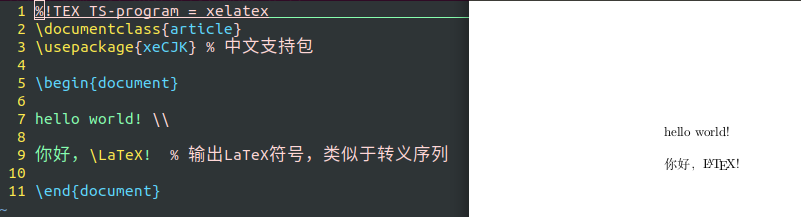
\includegraphics[scale=0.5]{1}
	\caption{a simple example of \LaTeX }
\end{figure}

	

可以看到,\%\ 后面的内容并没有输出,这就类似于程序设计中的注释一样。上面的
\ $\backslash\backslash$\ 用于换行。

\end{document}
